In this section, the models described in this report are compared with the performance profile tool provided. Several runs were carried out to fully test the models for a more accurate conclusion. In particular, the best algorithm is the one that finds the optimal solution in the shortest time for most of the time. While analyzing the metaheuristics approaches it is impossible to compare them in a time scale, so instead of the time the comparison here is done between the cost of the solution obtained.

Since the TSP is a NP-hard problem, finding a winner is not always easy. Sometimes different methods can lead to very similar results, so several factors - such as consistency - are took in consideration.

To discuss, the outcome of the tests is plotted and so it is needed some explanation on how to understand them. While the x-axis portrays the time (or cost) ratio which will show what algorithm performs better, the y-axis shows the fraction of instances that the algorithm ends up winning. In general, the best method is the one that remains more on the left side of the chart.

As explained in section \ref{sec:solution-data-management}, the TSPLIB is used only to carry out if the implemented algorithms can reach the optimal value. To run these tests, a series of randomly generated instances are used.

\section{Compact models}
\label{sec:results-compact}
In this section the compact models presented in chapter \ref{chapter:compact-models} focusing in particular of MTZ and its variants and GG models. To test them a set of 20 instance of 50 nodes were generated and runned with a global timelimit of 30 minutes. The results are visible in figure \ref{fig:result-compact}.

\begin{figure}[h]
	\centering
	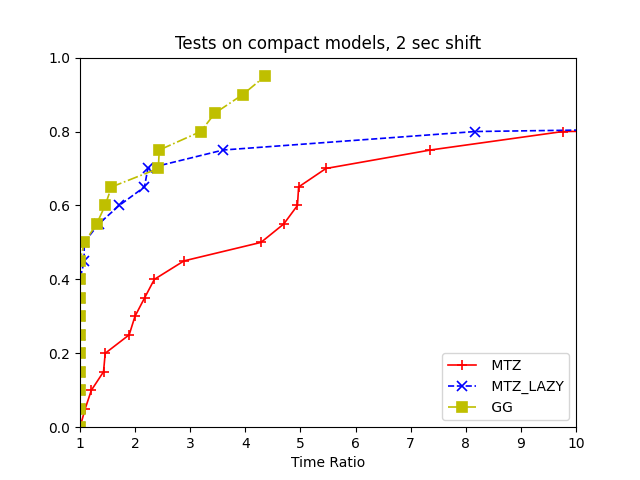
\includegraphics[width=0.6\textwidth]{images/final_mtz_mtzlazy_gg.png}
	\caption{The comparison chart of the compact models.}
	\label{fig:result-compact}
\end{figure}

From this image we can state that the MTZ basic model is far from being the best one of this section. In fact the best models are GG and MTZ\_LAZY wich on many instaces perform in a comparable way. But it is possible to see that while MTZ\_LAZY in some cases as reached the timelimit, the GG model deliver a consistent solution of the instance.

\section{SEC methods}
\label{sec:results-sec}
To test the algorithms presented in section \ref{chapter:other-sec}, a set of 20 instances with 350 nodes was created.

\begin{figure}[h]
	\centering
	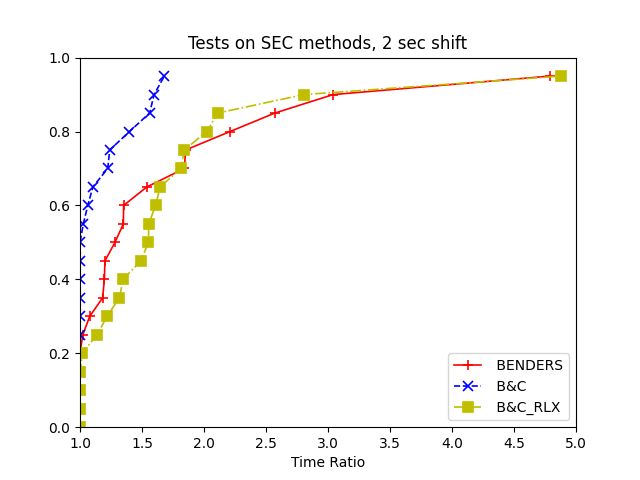
\includegraphics[width=0.6\textwidth]{images/final_SEC.png}
	\caption{The comparison chart of the SEC methods.}
	\label{fig:result-sec}
\end{figure}

The results in figure \ref{fig:result-sec} showed clearly that the Branch and Cut method is the best approach of this comparison. The most outstanding outcome is that the B\&C (Branch-and-Cut) relaxation method was in a trailing position even compared with the Benders method, while I was assuming that its performance was comparable with the normal B\&C.

The meaning of this is the fact that the callback is applied each time a fractional solution is found. This suggests that it is called way more times than in the previous one and this leads to worse performance. For solving this problem, I have done deeper research on this approach. Figure \ref{fig:result-bac} shows the B\&C relaxation applied with a different probability.

\begin{figure}[h]
	\centering
	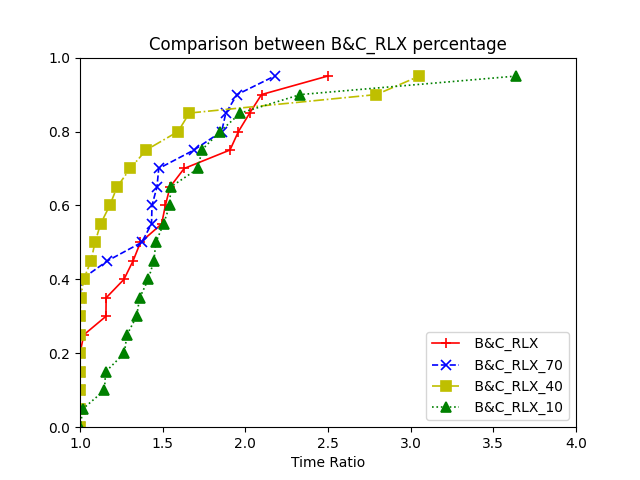
\includegraphics[width=0.6\textwidth]{images/branch_perc.png}
	\caption{The comparison between different B\&C relaxation.}
	\label{fig:result-bac}
\end{figure}

This plot shows that the best performing method is the one with a percentage of 40\%. In this way is possible to obtain the final chart with the best methods.

\begin{figure}[h]
	\centering
	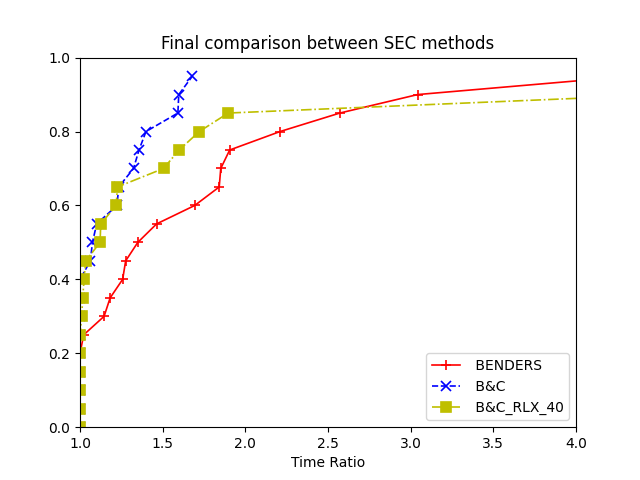
\includegraphics[width=0.6\textwidth]{images/final_final_SEC.png}
	\caption{Final comparison between different B\&C.}
	\label{fig:result-final-bac}
\end{figure}

This last chart shows that the classic Branch and Cut method and the relaxation one applied with a percentage of 40\% are similar, but the one that solves only the integer solution is considered the best among them.



\section{Matheuristics}
\label{sec:results-math}
"The objective of a heuristic is to produce a solution in a reasonable time frame that is good enough for solving the problem at hand. This solution may not be the best of all the solutions to this problem, or it may simply approximate the exact solution. But it is still valuable because finding it does not require a prohibitively long time"\cite{heuristic}.\\
The two techniques I am going to delve into are the hard-fixing and the soft-fixing.

\subsection{Hard-fixing}
\label{section:hard-fix}
The main purpose of this method is to try to reduce the search space by cutting down the complexity of the optimization. For achieving this goal, an initial feasible solution is needed - obtained by any approach described in this report.\\
The central thought of hard-fixing is to get an easier problem by setting some variables of the solution passed to the method - and so by having fewer variables to compute. The variables to be fixed are $x_{ij}$, $i, j\in V$. This task is done by settling the values to 1, so that the edge will be surely part of the solution. A valid method to choose which path is designated to be fixed is to link each edge to a probability $p$ between $0$ and $1$, then set randomly - with the probability picked - the value to 1.\\
Hereupon, the problem will presumably have $p*|E|$ variables fixed and thus the instance can be solved with a lower effort. Hopefully, this situation will bring to a better solution. Although the choice of using a probability is a good pick, any other method can be used to block the edges.

The performance of this technique is strictly related to the choice of the first feasible solution: if it is not good enough, this approach will get stuck on some non-optimal solution. A good fix for avoiding this is to lower down $p$ whenever the solution is not improved for a predetermined amount of time.

\begin{algorithm}
	\caption{Hard-fixing}\label{algo:hard-fix}
	\begin{algorithmic}[1]
		\Require $G=(V,E)$,$ c:E\rightarrow \Re^+$, $global\_timelimit$, $iteration\_timelimit$
		\Ensure $z\text{ hopefully good solution}$
		\State instance $\gets$ *initializing model (any of this report)*
		
		\State  $z$ $\gets$ \textsc{CPXmipopt} *with nodelimit 0*
		\State $p$ $\gets$ $0.9$
		\State $i$ $\gets$ $0$
		\While{$time\_elapsed<global\_time\_limit$}
			\If{$time\_remaining > iteration\_timelimit$}
				\State instance $\gets$ *set timelimit to $iteration\_timelimit$*
			\Else 
				\State instance $\gets$ *set timelimit to $time\_remaining$*
			\EndIf
			\State instance $\gets$ *hard-fixing with probability $p$*
			\State $z_{new}$ $\gets$ \textsc{CPXmipopt}
			
			\If{$cost(z_{new})<cost(z)$}
				\State $z$ $\gets$ $z_{new}$
				\State $i$ $\gets$ $0$
			\Else 
				\State $i$ $\gets$ $i+1$
			\EndIf
			
			\If{$i = 10$}
				\State $p$ $\gets$ $p - 0.1$
			\EndIf
			\State instance $\gets$ *remove hard-fixing*
		\EndWhile
		\State \Return $z$
	\end{algorithmic}
\end{algorithm}

In this algorithm, there are some variables not mentioned before: the global timelimit and the iteration timelimit. As aforementioned, the hard-fixing is a technique that aims to obtain a good solution in a short amount of time, so the parameters described above are necessary to establish - as the name suggests - the timespan in which the optimization is solved. global\_timelimit is the total time reserved to the solver, interation\_timelimit is the duration of each optimization in which the hard-fixing is applied.

The initial solution is provided by the solver, limited in the depth of its analysis. Then, algorithm \ref{algo:hard-fix} starts to iterate the main process until the global\_timelimit is reached. During this phase, the optimization is called several times, in each of which the instance is solved blocking some variables to $1$.

\subsection{Soft-fixing}
The technique that will be described is called Local Branching. Since it is a slight modification of the hard-fixing it is also called soft-fixing.\\
In section \ref{section:hard-fix} the value of the variables is fixed in a manual way using a probability system. In Local Branching, this operation is performed by adding a new constraint that forces the instance to block a predetermined number of variables, giving to the solver a degree of freedom on which variables to fix and which not.

The main idea of soft-fixing is the Hamming distance: "it measures the minimum number of substitutions required to change one string into the other"\cite{hamming-distance}. This description can be applied also to vectors. So given two vectors $x$ and $\tilde{x}$ in $\{0,1\}$, the Hamming distance is the number of different bits they have. It can be described in this way:

\begin{equation}
\label{eqn:hamming-dist}
H(x, \tilde{x}) = \sum_{j:\tilde{x}_j=1}(1-x_j)+\sum_{j:\tilde{x}_j=0}x_j
\end{equation}

Considering that the output solution of the solver is a vector in $\{0, 1\}$, it is possible to insert into the instance a new constraint that limits the hamming distance between the old solution and the new one.
The number of edges active in each solution is forced to be $n=|V|$ and therefore the Hamming distance is computed on the differences in the bits equal to 1. For this reason, it is possible to reduce \ref{eqn:hamming-dist} to:

\begin{equation}
\label{eqn:hamming-dist-2}
H(x, \tilde{x}) = \sum_{j:\tilde{x}_j=1}(1-x_j) =  n - \sum_{j:\tilde{x}_j=1}x_j
\end{equation}

The purpose of this method is to limit the diversity of two solutions. For doing so, it is possible to add a new variable $k$ that limits the Hamming distance. Through elementary math, this formulation is built as:

\begin{equation}
\label{eqn:hamming-dist-3}
H(x, \tilde{x}) \le k \Rightarrow n - \sum_{j:\tilde{x}_j=1}x_j \le k \Rightarrow \sum_{j:\tilde{x}_j=1}x_j \ge n - k
\end{equation}

The consequence of \ref{eqn:hamming-dist-3} is to narrow the next iteration of the optimization to a $k$-neighborhood of the previous one. As the method described in section \ref{section:hard-fix}, the value $k$ can vary if for the optimization doesn't improve the solution. 

\begin{algorithm}
	\caption{Soft-fixing}\label{algo:soft-fix}
	\begin{algorithmic}[1]
		\Require $G=(V,E)$,$ c:E\rightarrow \Re^+$, $global\_timelimit$, $iteration\_timelimit$
		\Ensure $z\text{ hopefully good solution}$
		\State instance $\gets$ *initializing model (any of this report)*
		
		\State  $z$ $\gets$ \textsc{CPXmipopt} *with nodelimit 0*
		\State $k$ $\gets$ $2$
		\State $i$ $\gets$ $0$
		\While{$time\_elapsed<global\_time\_limit$}
		\If{$time\_remaining > iteration\_timelimit$}
		\State instance $\gets$ *set timelimit to $iteration\_timelimit$*
		\Else 
		\State instance $\gets$ *set timelimit to $time\_remaining$*
		\EndIf
		\State instance $\gets$ *soft-fixing using a k-neighborhood*
		\State $z_{new}$ $\gets$ \textsc{CPXmipopt}
		
		\If{$cost(z_{new})<cost(z)$}
		\State $z$ $\gets$ $z_{new}$
		\State $i$ $\gets$ $0$
		\Else 
		\State $i$ $\gets$ $i+1$
		\EndIf
		
		\If{$i = 10$}
		\State $k$ $\gets$ $k + 1$
		\EndIf
		\State instance $\gets$ *remove soft-fixing*
		\EndWhile
		\State \Return $z$
	\end{algorithmic}
\end{algorithm}

The only changes between \ref{algo:hard-fix} and \ref{algo:soft-fix} are the variables used and the constraints added to the instance. In this implementation, $k$ is increased by $1$ every time the solution is not improved.

\section{Metaheuristics}
\label{sec:results-heur}
This is the last comparison between the methods presented in this project. In this section, metaheuristics presented in chapter \ref{chapter:metaheuristics} are compared: the VNS, the Tabu Search, and the Genetic algorithms.

To compare them, larger instances than the previous ones are created. A set of 20 instances with 2000 nodes is randomly built and then they are tested with a time limit of 30 minutes. The results are visible in figure \ref{fig:result-meta}.

\begin{figure}[h]
	\centering
	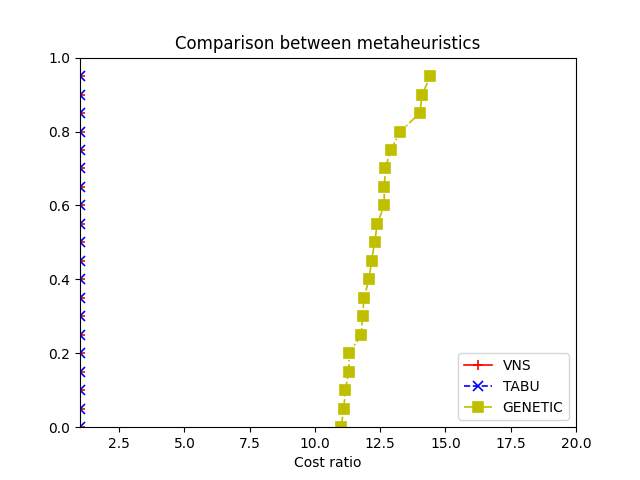
\includegraphics[width=0.6\textwidth]{images/final_meta.png}
	\caption{The comparison between the Matheuristics.}
	\label{fig:result-meta}
\end{figure}

It is possible to notice that genetic algorithms lead to worst solutions. This is due to the fact that the starting population is totally randomly generated and so, within a small time limit, it is difficult to improve as much as in VNS or Tabu Search.

To see the winner of this section it is necessary to zoom the left side of the chart. 

\begin{figure}[h]
	\centering
	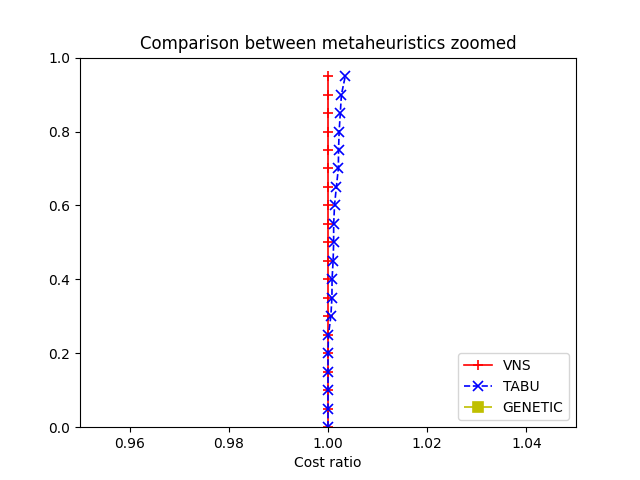
\includegraphics[width=0.6\textwidth]{images/final_meta_zoom.png}
	\caption{The comparison between the Matheuristics.}
	\label{fig:result-meta-zoom}
\end{figure}

In figure \ref{fig:result-meta-zoom} it is evident that the winner of this comparison is the VNS.

\section{Conclusions}
\label{sec:conclusions}
Among all the exact algorithms there is no doubt that the best performing one is the B\&C method, which reached the optimal solution in the shortest amount of time. Given a sufficient time limit, it should be able to solve larger instances with enough efficiency.

The use of a compact model is infeasible since the effort to compute an optimal solution is enormous and surely not worth it. However in this category, the best performing one is the GG model because it delivers consistently an optimal solution.

By all the matheuristic approaches the best-performing one was the Soft-Fixing, which brings the best solution most of the time. The Hard-Fixing method is still usable though because the solutions obtained from it are not too far away from the best ones.

The best metaheuristic approach is the VNS, which always provides the better solution. The use of the Soft-Fixing method is possible even with a higher number of nodes but - given a short amount of time - the solver hardly reaches a feasible solution.